%%%%%%%%%%%%%%%%%%%%%%%%%%% COORDINATESYSTEMS
% COORDSYS (ORIGOCOORDINATENAME, WIDTH, HEIGHT)
% Draws a Coordinatesystem around ORIGOCOORDINATENAME with a width of WIDTH and a height of HEIGHT, 
% names the beginning and end of axes, southwest corner, northwest corner, 
\newcommand{\CoordSys}[3]{
\coordinate (XY#1) at ([xshift=#2 cm, yshift=#3 cm]#1);
\coordinate (-XY#1) at ([xshift=-#2 cm, yshift=-#3 cm]#1);
\coordinate (-X#1) at ([xshift=-#2 cm]#1);
\coordinate (X#1) at ([xshift=#2 cm]#1);
\coordinate (Y#1) at ([yshift=#3 cm]#1);
\coordinate (-Y#1) at ([yshift=-#3 cm]#1);
\draw [help lines, step=.5cm] (-XY#1) grid (XY#1);
\draw[->] (-X#1)--(X#1);
\draw[->] (-Y#1)--(Y#1);
}

%Lorentz(OriginalOriginCoord, ResultingOriginCoord, SpeedNum, PointCoord, Label)
% 
\newcommand{\Lorentz}[5]{
\path (#1); \pgfgetlastxy{\XCoord}{\YCoord}; % Extracting coordinates of the Origin
\pgfmathsetmacro{\XOrigin}{\XCoord} % Saving X coordinate
\pgfmathsetmacro{\YOrigin}{\YCoord} % Saving Y coordinate
\path (#4); \pgfgetlastxy{\XCoord}{\YCoord}; % Extracting coordinates of the Point
\pgfmathsetmacro{\XEvent}{\XCoord} % Saving X coordinate
\pgfmathsetmacro{\YEvent}{\YCoord} % Saving Y coordinate
\pgfmathsetmacro{\XEventWRTOrigin}{\XEvent-\XOrigin} % Relativizing to the origin
\pgfmathsetmacro{\YEventWRTOrigin}{\YEvent-\YOrigin} % Relativizing to the origin
\pgfmathparse{XLorentz(#3,\XEventWRTOrigin,\YEventWRTOrigin)} % transforming x
\pgfmathsetmacro{\XEventTr}{\pgfmathresult} % save the result of x
\pgfmathparse{YLorentz(#3,\XEventWRTOrigin,\YEventWRTOrigin)} % transforming y
\pgfmathsetmacro{\YEventTr}{\pgfmathresult} % save the result of y
\node[world](#5) at (
[xshift=\XEventTr pt,
 yshift=\YEventTr pt] #2){};
}

\usetikzlibrary{calc}
\newdimen\XCoord
\newdimen\YCoord

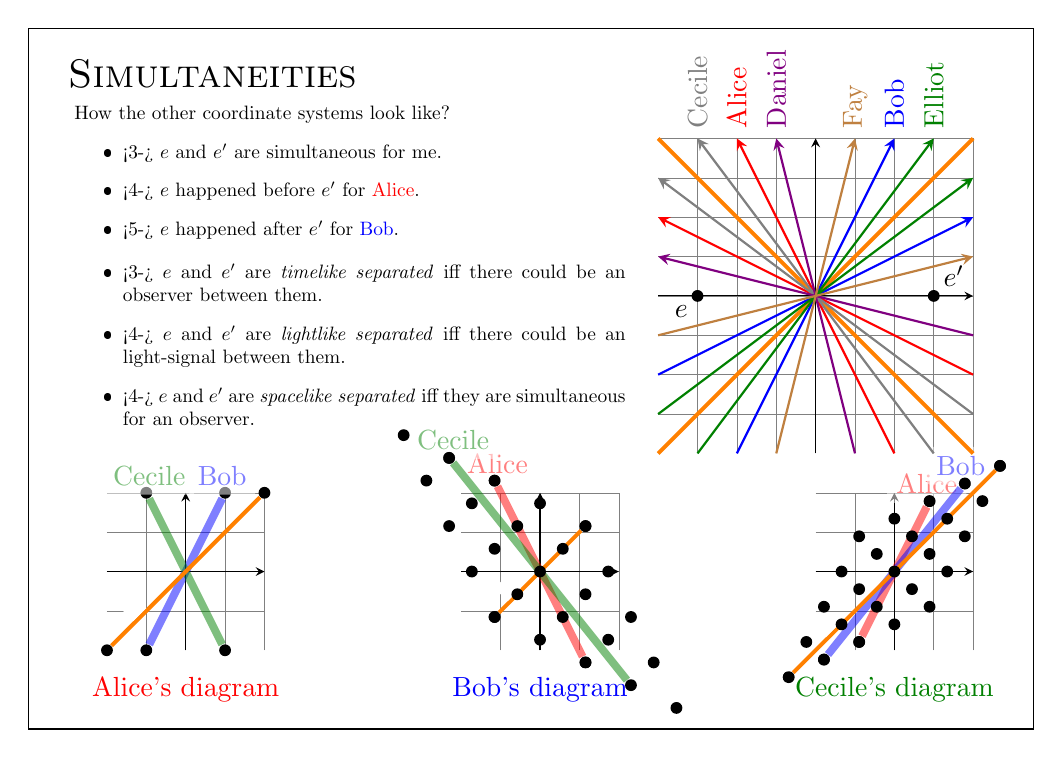
\begin{tikzpicture}[>=stealth, scale=1,
world/.style={inner sep=0, minimum size=.15cm, fill=black, circle},
worldline/.style={line width=1mm, rounded corners=1pt, opacity=.5},
axis/.style={->},
light/.style={orange, line width=.5mm},
]
\pgfmathdeclarefunction{XLorentz}{3}{\pgfmathparse{(#2 - #1*#3)/(sqrt(1-#1^2))}} % speed, spacecoord, timecoord
\pgfmathdeclarefunction{YLorentz}{3}{\pgfmathparse{(#3 - #1*#2)/(sqrt(1-#1^2))}} % speed, spacecoord, timecoord

%%%%%%%%%%%%%%%%%%%%%%%% DIA KEZDETE %%%%%%%%%%%%%%%%%%%%%%%%%%%

\node[anchor=north west, inner sep=0] at (0.5,8.5) {\textsc{\Large Simultaneities}}; %%%%%%% TITLE
%\node[anchor=north west, inner sep=0] at (0.5,8) {\textsc{\normalsize Role of Light}}; %%%%%%% SUBTITLE
\draw%[white]  %%%%%%%%%%%% SIZE OF THE SLIDE
      (0,0) rectangle (12.77,8.9);
%%%%%%%%% TEXT %%%%%%%%%%%%%
\node[anchor=north west, scale=.7] at (0.5,8) {\begin{minipage}{10cm}
How the other coordinate systems look like?
\begin{itemize}
\item<3-> $e$ and $e'$ are simultaneous for me.
\item<4-> $e$ happened before $e'$ for \textcolor{red}{Alice}.
\item<5-> $e$ happened after $e'$ for \textcolor{blue}{Bob}.
\end{itemize}
\begin{itemize}
\item<3-> $e$ and $e'$ are \emph{timelike separated} iff there could be an observer between them.
\item<4-> $e$ and $e'$ are \emph{lightlike separated} iff there could be an light-signal between them.
\item<4-> $e$ and $e'$ are \emph{spacelike separated} iff they are simultaneous for an observer.
\end{itemize}
\end{minipage}
};
%%%%%%%%%%%%%%%%%%%%%%%% KOORDINÁTARENDSZEREK %%%%%%%%%%%%%%%%%%%%%%%%%%%
\coordinate(O1) at (2,2) {} {};
  \CoordSys{O1}{1}{1}
\coordinate(O2) at (6.5,2) {} {};
  \CoordSys{O2}{1}{1}
\coordinate(O3) at (11,2) {} {} {};
  \CoordSys{O3}{1}{1}

\coordinate(O4) at (10,5.5) {} {} {} {} {};
  \CoordSys{O4}{2}{2}

%%%%%%%%%%
%% SETTINGS %%
%%%%%%%%%%


\coordinate (SignalStart) at (1,1) {} {} {};
\coordinate (SignalBounced) at (3,3) {} {} {};
\coordinate (AliceStart) at (2,1) {} {} {};
\coordinate (AliceEnd) at (2,3) {} {} {};
\coordinate (BobStart) at (1.5,1) {} {} {} {} {} {}; % Fontos hogy átmenjen az Origón, különben rossz a lorentz transzformáció!!
\coordinate (BobEnd) at (2.5,3) {} {} {} {} {} {};
\coordinate(CecileEnd) at (1.5,3) {};
\coordinate(CecileStart) at (2.5,1) {};

%%%%%%%%%%% Ezt lehetne macronak, speedszámítócuccnak
\path (BobStart); \pgfgetlastxy{\XCoord}{\YCoord}; % Extracting coordinates of the Origin
\pgfmathsetmacro{\XFirst}{\XCoord} % Saving X coordinate
\pgfmathsetmacro{\YFirst}{\YCoord} % Saving Y coordinate
\path (BobEnd); \pgfgetlastxy{\XCoord}{\YCoord}; % Extracting coordinates of the Point
\pgfmathsetmacro{\XSecond}{\XCoord} % Saving X coordinate
\pgfmathsetmacro{\YSecond}{\YCoord} % Saving Y coordinate
\pgfmathsetmacro{\SpeedBob}{(\XFirst-\XSecond)/(\YFirst-\YSecond)} % Relativizing to the origin
%%%%%%%%%%%%%%%%%%%%%%%%%%%%%%%%%%%

\Lorentz{O1}{O1}{0}{BobStart}{BS}
\Lorentz{O1}{O1}{0}{BobEnd}{BE}
\Lorentz{O1}{O1}{0}{CecileStart}{CS}
\Lorentz{O1}{O1}{0}{CecileEnd}{CE}
\Lorentz{O1}{O1}{0}{SignalStart}{SS}
\Lorentz{O1}{O1}{0}{SignalBounced}{SB}
\Lorentz{O1}{O2}{\SpeedBob}{AliceStart}{AS'}
\Lorentz{O1}{O2}{\SpeedBob}{AliceEnd}{AE'}
\Lorentz{O1}{O2}{\SpeedBob}{CecileStart}{CS'}
\Lorentz{O1}{O2}{\SpeedBob}{CecileEnd}{CE'}
\Lorentz{O1}{O2}{\SpeedBob}{SignalStart}{SS'}
\Lorentz{O1}{O2}{\SpeedBob}{SignalBounced}{SB'}
\Lorentz{O1}{O3}{-\SpeedBob}{AliceStart}{AS''}
\Lorentz{O1}{O3}{-\SpeedBob}{AliceEnd}{AE''}
\Lorentz{O1}{O3}{-\SpeedBob}{BobStart}{BS''}
\Lorentz{O1}{O3}{-\SpeedBob}{BobEnd}{BE''}
\Lorentz{O1}{O3}{-\SpeedBob}{SignalStart}{SS''}
\Lorentz{O1}{O3}{-\SpeedBob}{SignalBounced}{SB''}
\node[rotate=0, text=red, fill=white] at (2,0.5) {Alice's diagram};
\node[rotate=0, text=blue, fill=white] at (6.5,0.5) {Bob's diagram};
\node[rotate=0, text=green!50!black, fill=white] at (11,0.5) {Cecile's diagram};
\draw[worldline, blue] (BS)--(BE) node[fill=white, above, pos=1]{Bob};
\draw[worldline, green!50!black] (CS)--(CE) node[fill=white, above, pos=1]{Cecile};
\draw[worldline, red] (AS')--(AE') node[fill=white, above, pos=1]{Alice};
\draw[worldline, green!50!black] (CS')--(CE') node[fill=white, above, pos=1]{Cecile};
\draw[worldline, red] (AS'')--(AE'') node[fill=white, above, pos=1]{Alice};
\draw[worldline, blue] (BS'')--(BE'') node[fill=white, above, pos=1]{Bob};
\draw[light]  (SS)-- (SB) node[fill=white, sloped, above, pos=.2]{};
\draw[light]  (SS')-- (SB') node[fill=white, sloped, above, pos=.2]{};
\draw[light]  (SS'')-- (SB'') node[fill=white, sloped, above, pos=.2]{};

\foreach \x in {1, 1.5, ..., 3}
{\foreach \y in {1, 1.5, ..., 3}
 { %\coordinate(\x\y) at (\x,\y);
   \Lorentz{O1}{O2}{\SpeedBob}{\x,\y}{}
   \Lorentz{O1}{O3}{-\SpeedBob}{\x,\y}{}
 }}

\coordinate (v1) at (10.5,7.5) {} {};
\coordinate (v2) at (12,6) {} {};
\coordinate (v3) at (11,7.5) {} {};
\coordinate (v4) at (12,6.5) {} {};
\coordinate (v5) at (11.5,7.5) {} {};
\coordinate (v6) at (12,7) {} {};
\coordinate (v7) at (9.5,3.5) {} {};
\coordinate (v8) at (8,5) {} {};
\coordinate (v9) at (9,3.5) {} {};
\coordinate (v10) at (8,4.5) {} {};
\coordinate (v11) at (8.5,3.5) {} {};
\coordinate (v12) at (8,4) {} {};
\coordinate (v15) at (12,5) {} {};
\coordinate (v13) at (10.5,3.5) {} {};
\coordinate (v19) at (12,4.5) {} {};
\coordinate (v17) at (11,3.5) {} {};
\coordinate (v23) at (12,4) {} {};
\coordinate (v21) at (11.5,3.5) {} {};
\coordinate (v14) at (9.5,7.5) {} {};
\coordinate (v16) at (8,6) {} {};
\coordinate (v18) at (9,7.5) {} {};
\coordinate (v20) at (8,6.5) {} {};
\coordinate (v22) at (8.5,7.5) {} {};
\coordinate (v24) at (8,7) {} {};
\coordinate (v25) at (8,3.5) {} {} {};
\coordinate (v26) at (12,7.5) {} {} {};
\coordinate (v28) at (8,7.5) {} {} {};
\coordinate (v27) at (12,3.5) {} {} {};
\draw[light]  (v25) edge (v26);
\draw[light]  (v27) edge (v28);
\begin{scope}[->, thick]
%\pause
\draw[red]  (v17) -- (v18);
\draw[red]  (v19) -- (v20);
\node[red, anchor=west, rotate=90] at (v18) {Alice};
%\pause
\draw[blue]  (v9) -- (v3);
\draw[blue]  (v10) -- (v4);
\node[blue, anchor=west, rotate=90] at (v3) {Bob};
%\pause
\draw[gray]  (v21) -- (v22);
\draw[gray]  (v23) -- (v24);
\node[gray, anchor=west, rotate=90] at (v22) {Cecile};
%\pause
\draw[violet]  (v13) -- (v14);
\draw[violet]  (v15) -- (v16);
\node[violet, anchor=west, rotate=90] at (v14) {Daniel};
%\pause
\draw[green!50!black]  (v11) -- (v5);
\draw[green!50!black]  (v12) -- (v6);
\node[green!50!black, anchor=west, rotate=90] at (v5) {Elliot};
%\pause
\draw[brown]  (v7) -- (v1);
\draw[brown]  (v8) -- (v2);
\node[brown, anchor=west, rotate=90] at (v1) {Fay};
\end{scope}
\node[world](e) at (8.5,5.5) {};
\node[anchor=north east] at (e){$e$};
\node[world](e') at (11.5,5.5) {};
\node[anchor=south west] at (e'){$e'$};
\end{tikzpicture}